\section{Dataset / Input Description}
The system uses a video-based dataset consisting of Indian Sign Language gestures. Each sample in the dataset represents a gesture performed by a signer.

\begin{itemize}[leftmargin=1.5em]
\item Input data consists of RGB video sequences,
\item Videos are converted into frames for processing,
\item Each sequence represents a single gesture class (isolated gestures),
\item Preprocessing ensures uniform frame size and sequence length.
\end{itemize}

The dataset and input representation are shown in Fig.~\ref{fig:dataset-input}.

\begin{figure}[H]
\centering
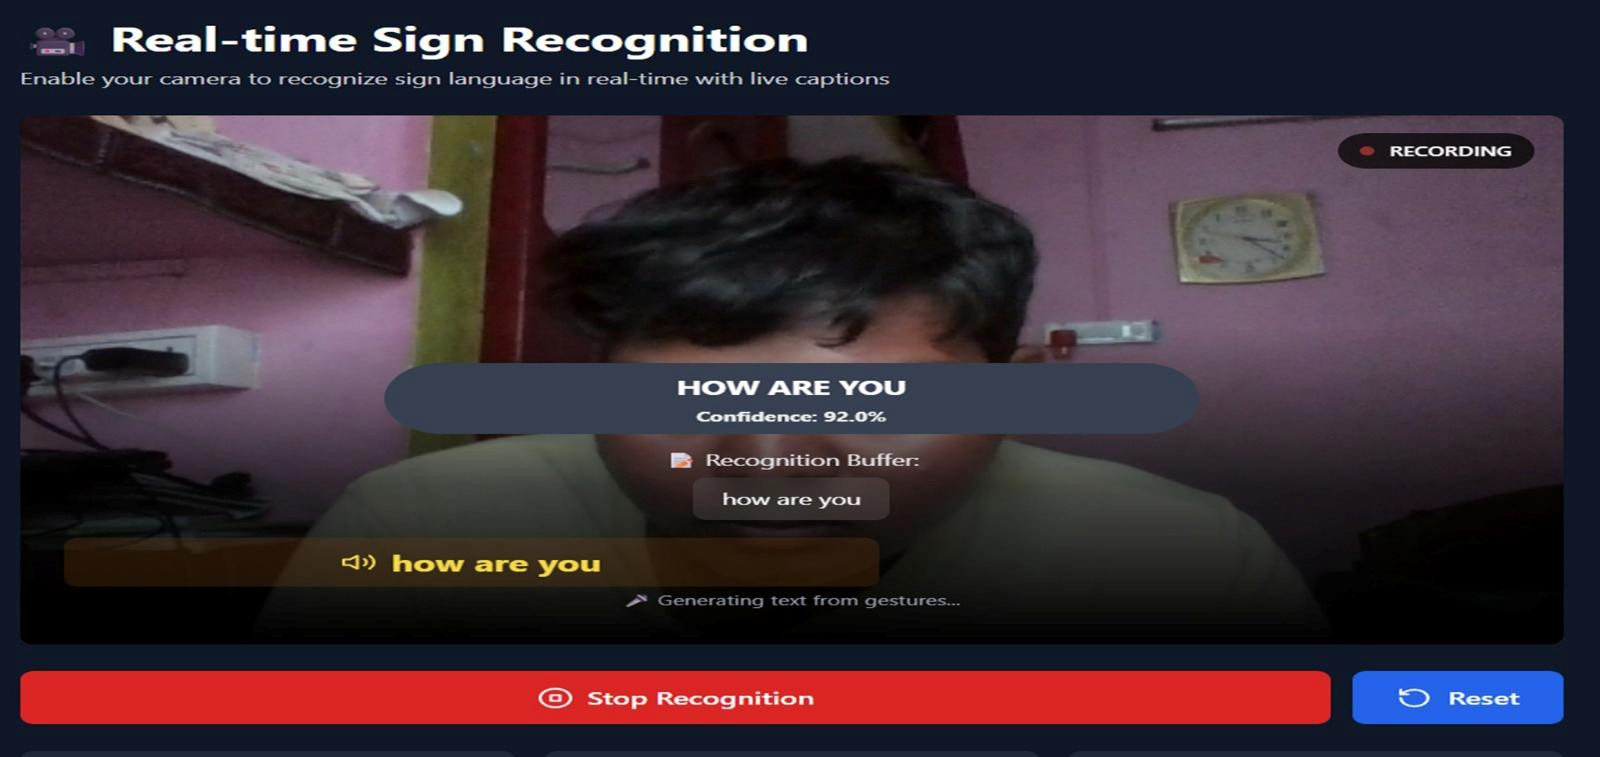
\includegraphics[width=0.9\textwidth]{text/figures/docx_image6.jpeg}
\caption{Dataset and input representation snapshot.}
\label{fig:dataset-input}
\end{figure}
